%!TEX encoding = UTF-8 Unicode
%!TEX root = ../lect-w06.tex

%%%

\Subsection{Typhierarkier i Scala}

\begin{Slide}{Bastypen för alla typer: \texttt{Any}}
\SlideFontSmall
Scalas typsystem är \Alert{fullständigt}:
\begin{itemize}\SlideFontSmall
  \item Alla värden är objekt som har en typ.
  \item Alla typer är subtyper till bastypen \code{Any}.
  \item Typen \code{Any} kallas därför \Emph{topptyp}.
  \item Alla objekt har vissa grundläggande metoder, så som \code{toString} och \code{==}
\begin{Code}
abstract class Any:   // en förenklad bild av innehållet i Any:
  def toString
  def ==
  def !=
  def equals
  def isInstanceOf
  def asInstanceOf
  def ##
  def hashCode
  def getClass

trait Matchable extends Any
\end{Code}
\end{itemize}

Det kommer mer om abstrakta klasser och traits i veckan om arv.
\end{Slide}

\begin{Slide}{Alla typer är subtyper till \texttt{Any}}\SlideFontSmall\ifkompendium\footnotesize\fi
\vspace{-0.0em}\begin{center}
\newcommand{\TextBox}[1]{\raisebox{0pt}[1em][0.5em]{#1}}
\tikzstyle{umlclass}=[rectangle, draw=black,  thick, anchor=north, text width=2cm, rectangle split, rectangle split parts = 3]
\begin{tikzpicture}[inner sep=0.5em]
\node [umlclass, rectangle split parts = 1, xshift=0cm] (Any)  {
            \textit{\textbf{\centerline{\TextBox{\code{Any}}}}}
        };

\node [umlclass, rectangle split parts = 1, yshift=-1.5cm] (Matchable)  {
            \textit{\textbf{\centerline{\TextBox{\code{Matchable}}}}}
        };



\node [umlclass, rectangle split parts = 1]  at (-2.5cm,-3.25cm) (SubType1) {
            \textbf{\centerline{\TextBox{\code{AnyVal}}}}
            % \nodepart[]{second} \TextBox{\code{val x: A}}
        };

\node [umlclass, rectangle split parts = 1] at (2.5cm,-3.25cm) (SubType2)  {
            \textbf{\centerline{\TextBox{\code{AnyRef}}}}
        };

\draw[umlarrow] (Matchable.north) -- ++(0,0.5) -| (Any.south);
\draw[umlarrow] (SubType1.north) -- ++(0,0.5) -| (Matchable.south);
\draw[umlarrow] (SubType2.north) -- ++(0,0.5) -| (Matchable.south);
\end{tikzpicture}
\end{center}
\begin{itemize}
  \item Alla \Emph{värdetyper}, t.ex. \code{Int}, \code{Double}, \code{Boolean}, är subtyper till \code{AnyVal}
  \item Alla \Emph{referenstyper} t.ex. \code{String} är subtyper till \code{AnyRef}
  \item Värden av typen \code{Matchable} kan användas vid s.k mönstermatchning. 
  \item (Det finns även s.k. opaka typer som inte kan mönstermatchas.)
\end{itemize}
\end{Slide}

\begin{Slide}{Dina egna referenstyper är subtyper till \texttt{AnyRef}}\SlideFontSmall
Alla typer du skapar är subtyper till \code{AnyRef} utan att du behöver skriva det.
\begin{Code}
trait Grönsak:                                 // din egen bastyp
  def vikt: Int

case class Gurka(vikt: Int) extends Grönsak    // din egen subtyp
case class Tomat(vikt: Int) extends Grönsak    // en annan subtyp
\end{Code}
\SlideFontSmall\ifkompendium\footnotesize\fi
\vspace{-0.0em}\begin{center}
\newcommand{\TextBox}[1]{\raisebox{0pt}[1em][0.5em]{#1}}
\tikzstyle{umlclass}=[rectangle, draw=black,  thick, anchor=north, text width=2cm, rectangle split, rectangle split parts = 3]
\begin{tikzpicture}[inner sep=0.5em]
\node [umlclass, rectangle split parts = 1, yshift=-1.5cm] (Base)  {
            \textit{\textbf{\centerline{\TextBox{\code{Grönsak}}}}}
        };



\node [umlclass, rectangle split parts = 1]  at (-2.5cm,-3.5cm) (SubType1) {
            \textbf{\centerline{\TextBox{\code{Gurka}}}}
            % \nodepart[]{second} \TextBox{\code{val x: A}}
        };

\node [umlclass, rectangle split parts = 1] at (2.5cm,-3.5cm) (SubType2)  {
            \textbf{\centerline{\TextBox{\code{Tomat}}}}
        };

\draw[umlarrow] (SubType1.north) -- ++(0,0.5) -| (Base.south);
\draw[umlarrow] (SubType2.north) -- ++(0,0.5) -| (Base.south);
\end{tikzpicture}
\end{center}
Det kommer mer om typhierarkier och \code{extends} i veckan om arv.
\end{Slide}

\Subsection{Mönstermatchning}

\ifkompendium
\noindent  I ett match-uttryck kan man matcha på ett visst värde eller på en viss typ och match-uttryck används gärna istället för nästlade if-uttryck, då de ofta är lättare att läsa och begripa. Med match-uttryck kan man också göra \Emph{mönstermatchning} mot case-klass-instanser, t.ex. för att på ett smidigt sätt undersöka om attribut har speciella värden. Match-uttryck i Scala är en mer kraftfull variant av \code{switch}-satser som finns i många andra språk.  
\fi

\begin{Slide}{Vad är matchning?}

  \begin{itemize}
    \item Matchning gör man då man vill jämföra ett värde mot andra värden och hitta överensstämmelse \Eng{match} enligt olika \Emph{mönster}.
    \item Med mönster kan man även \Alert{plocka isär} objekt i sina beståndsdelar.
  \end{itemize}
\end{Slide}

\begin{Slide}{Plocka isär ett objekt i sina beståndsdelar med mönster}

\begin{REPLnonum}
scala> case class Point(x: Int, y: Int)

scala> val p = Point(1, 2)      // konstruera en punkt
val p: Point = Point(1,2)
\end{REPLnonum}

\pause 

\begin{REPLnonum}
scala> val Point(x, y) = p      // plocka isär en punkt
val x: Int = 1
val y: Int = 2
\end{REPLnonum}
\pause \code{Point(x, y)} kallas ett \Emph{konstruktormönster}.\\ Namnen \code{x} och \code{y} blir nya variabler.\\ Det finns många olika sorters mönster. \\
Vanligaste användningen av mönster är i \code{match}-uttryck.
\end{Slide}


\begin{Slide}{Kolla om det passar med nästlade if-uttryck}
Ett vanligt problem: \\ att kolla vilket bland många värden som passar \\~\\

Kan göras med nästlade if-then-else-uttryck:

\begin{Code}
val g = scala.io.StdIn.readLine("Ange en grönsak:")
val smak =
  if g == "gurka" then "gott!"
  else if g == "tomat" then "jättegott!"
  else if g == "broccoli" then "ganska gott..."
  else "inte gott :("

println(g + " är " + smak)
\end{Code}
      
\end{Slide}


\ifkompendium\else
\begin{SlideExtra}{Matchning är ungefär som att passa klossar i en låda}
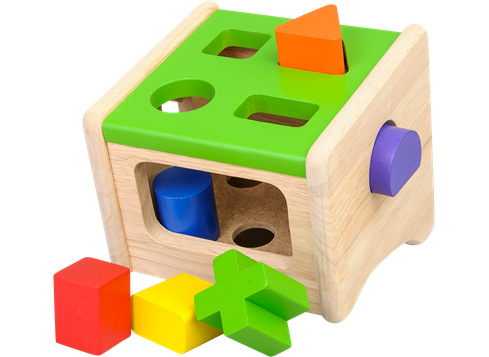
\includegraphics[width=0.8\textwidth]{../img/plocklada.png}
\end{SlideExtra}
\fi


\begin{Slide}{Kolla om det passar med \texttt{match}-uttryck}\SlideFontSmall
I stället för nästlade \code{if} kan du använda Scalas kraftfulla \code{match}-\Emph{uttryck}:

\begin{Code}
val g = scala.io.StdIn.readLine("Ange en grönsak: ")
val smak = g match 
  case "gurka"    => "gott!"
  case "tomat"    => "jättegott!"
  case "broccoli" => "ganska gott..."
  case _ => "mindre gott..."
\end{Code}
\begin{itemize}
\pause\item Varje \code{case}-gren testas var för sig i tur och ordning \Emph{uppifrån och ned}.
\item Det som står mellan \code{case} och \code{=>} kallas ett \Emph{mönster} \Eng{pattern}
\item Om ett mönster kan matchas så görs det som står efter \code{=>} 
\item \Alert{Inga grenar testas efter lyckad match}.  
\item Sista default-grenen ovan kallas \Emph{wildcard-mönster}: \code{case _ => }
\item Ovan är exempel på matchning mot \Emph{konstant-mönster}, \\ i detta fallet tre stycken strängkonstantmönster.
\item Det finns många andra sätt att skriva mönster.
\end{itemize}
% \pause Scalas \code{match} ''faller inte igenom'' som \code{switch}-satser som finns i många språk, t.ex. Java...

\end{Slide}

\begin{Slide}{Syntax för match-uttryck}
Ett \code{match}-uttryck består av godtyckligt många \code{case ... => ...}
\begin{Code}
  värdeAttUndersöka match 
    case mönster1 => resultat1
    case mönster2 => resultat2
    case mönster3 => resultat3
    case mönsterN => resultatN
\end{Code}
\begin{itemize}
  \item Varje resultat-uttryck kan bestå av många rader. 
  \item  Inga klammerparenteser behövs efter \code{=>} 
\end{itemize}
\vspace{1em}
Om många rader efter \code{case} så blir sista uttrycket resultatet. \\
Vi ska nu se exempel på många olika mönster 

\end{Slide}
  


\begin{Slide}{Matchning med gard}
Man kan stoppa in en s.k \Emph{gard} \Eng{guard} innan pilen \code{=>} för att villkora matchningen: (notera \code{if} utan \code{then})
\begin{Code}
val g = scala.io.StdIn.readLine("Ange en grönsak: ")
val smak = g match 
  case "gurka" if math.random() > 0.5 => "gott ibland!"
  case "tomat" => "jättegott!"
  case "broccoli" => "ganska gott..."
  case _ => "mindre gott..."
\end{Code}
\code{case}-grenen med gard ger bara en lyckad matchning \\ om uttrycket efter \code{if} är sant; annars provas nästa gren, etc.
\end{Slide}

\begin{Slide}{Matchning med variabelmönster}\SlideFontSmall
Om det finns ett namn efter \code{case} som börjar med liten begynnelsebokstav, blir detta namn en variabel som automatiskt binds till uttrycket före \code{match}:

\begin{Code}
val g = scala.io.StdIn.readLine("Ange en grönsak: ")
val smak = g match 
  case "gurka" if math.random() > 0.5 => "gott ibland!"
  case "tomat" => "jättegott!"
  case "broccoli" => "ganska gott..."
  case other => "smakar bakvänt: " + other.reverse
\end{Code}

Ett \Alert{enkelt} \Emph{variabelmönster}, så som \\ \code{case other => ...} \\ i exemplet ovan, matchar \Alert{allt}! \\\code{other} får alltså värdet av \code{g} om \code{g} \Alert{inte} är \code{"gurka"}, \code{"tomat"}, \code{"broccoli"}.

\end{Slide}


\begin{Slide}{Matchning med eller-mönster}\SlideFontSmall
Om man har samma utfall för olika grenar kan dessa slås ihop och mönstret separeras med vertikalstreck: \code{|}
\begin{Code}
val g = scala.io.StdIn.readLine("Ange en grönsak: ")
val smak = g match 
  case "gurka" => "gott"
  case "tomat" => "gott"
  case "lök"   => "gott"
  case _ => "inte gott"
\end{Code}

Mer koncist med eller-mönster:

\begin{Code}
val g = scala.io.StdIn.readLine("grönsak:")
val smak = g match 
  case "gurka" | "tomat" | "lök" => "gott"
  case _ => "inte gott"
\end{Code}



\end{Slide}





\begin{Slide}{Matchning med typade mönster}\SlideFontSmall
Med en typannotering efter en variabel får man ett \Emph{typat mönster} \Eng{typed pattern}. Om matchningen lyckas blir värdet \Alert{omvandlat} till den specifika typen och binds till variabeln.
\begin{Code}
def f = 
  if math.random() < 0.5 then 42 + math.random() 
  else s"gurka ${math.random()}"

val i = f match 
  case x: Double => x.round.toInt
  case s: String => s.length
\end{Code}
\code{f} får typen \code{Matchable} som är subtyp till \code{Any}. Vilken typ får \code{i}? \pause ~~\code{Int}
{\SlideFontTiny \\\vspace{0.5em} Matchning mot specifika typer enl. ovan används i idiomatisk Scala hellre än \code{isInstanceOf} och \code{asInstanceOf} men man kan göra motsvarande ovan så här:
\begin{Code}
val i2: Int =  
  val x = f
  if x.isInstanceOf[Double] then x.asInstanceOf[Double].round.toInt
  else if x.isInstanceOf[String] then x.asInstanceOf[String].length
  else throw scala.MatchError(x)
\end{Code}
}
\end{Slide}

\begin{Slide}{Typen \text{Matchable}}
\begin{itemize}\SlideFontSmall
\item
När ett uttryck inte kan ges en mer specifik typ så härleds \code{Matchable}, vilket visar att värdet kan undersökas med \code{match}.
\item Exempel: För de orelaterade typerna \code{String} och \code{Double} är den mest specifika typen som kan härledas \code{Matchable}.

\begin{REPLsmall}
scala> def f = if math.random() > 0.5 then 42 else "hej"
def f: Matchable
\end{REPLsmall}

\item Typen \code{Matchable} är nästan lika generell som topptypen \code{Any}. 
\item \code{Matchable} infördes i Scala 3 med \Emph{opaka typalias} som garanterat aldrig boxas men inte kan mönstermatchas. (Ingår ej i denna kurs.)
\item Fördjupning om \code{Matchable} och \code{opaque type} i Scala 3 finns här:
\\\url{https://dotty.epfl.ch/docs/reference/other-new-features}
\end{itemize}
\end{Slide}

\begin{Slide}{Konstruktormönster med case-klasser}\SlideFontSmall
En basklass med gemensamma delar och två subtyper:
\begin{Code}
trait Grönsak:
  def vikt: Int
  def ärRutten: Boolean

case class Gurka(vikt: Int, ärRutten: Boolean) extends Grönsak
case class Tomat(vikt: Int, ärRutten: Boolean) extends Grönsak
\end{Code}
\pause
Tack vare case-klasserna kan man använda \Emph{konstruktormönster} \Eng{constructor pattern} för att se vad som finns \Alert{inuti} en instans:
\begin{Code}
def testa(g: Grönsak): String = g match 
  case Gurka(v, false) => "gott, väger " + v
  case Gurka(_, true)  => "inte gott"
  case Tomat(v, r)     => (if r then "inte " else "") + s"gott, väger $v"
  case _ => s"okänd grönsak: $g"
\end{Code}

Konstruktormönster ''\Emph{plockar isär}'' det som matchas och binder variabler till de attribut som finns i case-klassens konstruktor.
\end{Slide}


\begin{Slide}{Plocka isär samlingar med djupa mönster}
\begin{itemize}
  \item Man kan plocka isär innehållet i en samling så här:
\begin{Code}
def visa(xs: Vector[Grönsak]): String = xs match
  case Vector()               => "tom grönsaksvektor"
  case Vector(Gurka(v, true)) => s"en rutten gurka som väger $v"
  case Vector(g)              => s"exakt en grönsak: $g"
  case Vector(g1, g2)         => s"exakt två grönsaker: $g1, $g2"
  case Vector(g, gs*)         => s"först en $g och sedan svansen: $gs"
\end{Code}
\item Vad händer om du byter ordning på 2:a och 3:e mönstret?
\item \code{Vector(g, gs*)} kan också skrivas som \code{g +: gs}
\end{itemize}
\end{Slide}

\begin{Slide}{Matchning på tupler}
Det går fint att plocka isär tupler med mönstermatchning:\footnote{\url{https://youtu.be/aboZctrHfK8}}
\begin{Code}
var pair = ("hej", 42)

pair match
  case (a, b) if b == 42 => s"livets mening är funnen: $a"
  case (_, b)            => s"fattas mening: $b"

\end{Code}

\end{Slide}

\begin{Slide}{Mönstermatchning och uppräkning med case-objekt}\SlideFontSmall
En bastyp och specifika singelobjekt av gemensam typ:
\begin{Code}
trait Färg
case object Spader  extends Färg // funkar utan case men vi vill ha najs toString
case object Hjärter extends Färg
case object Ruter   extends Färg
case object Klöver  extends Färg

def parallellFärg(f: Färg): Färg = f match
  case Spader  => Klöver
  case Klöver  => Spader
  case Hjärter => Ruter
\end{Code}
Vilken case-gren har vi glömt? Kan kompilatorn hjälpa oss?
\pause
\begin{REPL}
scala> parallellFärg(Ruter)
scala.MatchError: Ruter 
\end{REPL}
\Alert{Undantag vid körtid} \code{:(}
\end{Slide}

\begin{Slide}{Mönstermatchning och förseglade typer}\SlideFontSmall
Med nyckelordet \code{sealed} får vi en kompileringsvarning.
\begin{Code}
sealed trait Färg //tryck Alt+Enter i REPL för tolkning av flera rader ett svep
case object Spader  extends Färg
case object Hjärter extends Färg
case object Ruter   extends Färg
case object Klöver  extends Färg

def parallellFärg(f: Färg): Färg = f match 
  case Spader  => Klöver
  case Klöver  => Spader
  case Hjärter => Ruter
\end{Code}
\begin{REPL}
1 |def parallellFärg(f: Färg): Färg = f match 
  |                                   ^
  |                           match may not be exhaustive.
  |
  |                           It would fail on pattern case: Ruter
def parallellFärg(f: Färg): Färg
\end{REPL}
\Emph{Varning vid kompilering} \code{:)} ~~~Sista raden visar att det bara är en varning!
\end{Slide}

\begin{Slide}{Mönstermatcha enumeration}\SlideFontSmall
I stället för \code{sealed trait ... case object ...} kan du använda en \Emph{enumeration} (ä.k. uppräkning, uppräknad datatyp, \Eng{enumeration}).
\begin{Code}
enum Färg:
  case Spader, Hjärter, Ruter, Klöver
  
def parallellFärg(f: Färg): Färg = 
  import Färg.*
  f match 
    case Spader  => Klöver
    case Klöver  => Spader
    case Hjärter => Ruter
\end{Code}
\pause
\begin{REPL}
def parallellFärg(f: Färg): Färg
3 |  f match 
  |  ^
  |  match may not be exhaustive.
  |
  |  It would fail on pattern case: Ruter
\end{REPL}
\Emph{Även här får vi hjälpsam varning vid kompilering} \code{:)} 
\end{Slide}

\begin{Slide}{Stora/små begynnelsebokstäver vid matchning}
\Alert{Fallgrop}: matcha \Alert{värde} som börjar med \Alert{liten} bokstav.
\begin{REPL}
scala> val livetsMening = 42

scala> def ärLivetsMeningBuggig(svar: Int) = svar match 
         case livetsMening => true    // lokalt namn som matchar allt!
         case _ => false

scala> ärLivetsMeningBuggig(43)
val res0: Boolean = true

scala> val LivetsMening = 42   // stor begynnelsebokstav

scala> def ärLivetsMening(svar: Int) = svar match 
         case LivetsMening => true    // funkar fint!
         case _ => false

scala> ärLivetsMening(43)
val res1: Boolean = false
\end{REPL}
\end{Slide}


\begin{Slide}{Stora/små begynnelsebokstäver vid matchning}
Ett sätt att komma runt problemet med liten begynnelsebokstav: \\
\Emph{backticks} to the rescue!
\begin{REPL}
scala> val livetsMening = 42

scala> def ärLivetsMeningBackTicks(svar: Int) = svar match 
         case `livetsMening` => true    // nu funkar det!
         case _ => false

scala> ärLivetsMeningBackTicks(43)
val res2: Boolean = false
\end{REPL}
\end{Slide}

\ifkompendium\else
\begin{Slide}{Mönster på andra ställen än i \texttt{match}}\SlideFontSmall
Mönster i \Emph{deklarationer}:
\vspace{-0.25em}\begin{REPL}
scala> case class Point(x: Int, y: Int)

scala> val p = Point(0, 1)

scala> val Point(x, y) = p          // konstruktormönster med case-klass
val x: ???
val y: ???

scala> val (x, y, z) = (0, 1, 2)    // konstruktormönster med tupel
val x: ???
val y: ???
val z: ???

\end{REPL}
Mönster i \Emph{for-uttryck}:
\vspace{-0.25em}\begin{REPL}
scala> val xs = for (x, y) <- Vector((1,2), (3,4)) yield x
val xs: ???
\end{REPL}

\end{Slide}
\fi

\begin{Slide}{Mönster på andra ställen än i \texttt{match}}\SlideFontSmall
Mönster i \Emph{deklarationer}:
\vspace{-0.25em}\begin{REPL}
scala> case class Point(x: Int, y: Int)

scala> val p = Point(0, 1)

scala> val Point(x, y) = p          // konstruktormönster med case-klass
val x: Int = 0
val y: Int = 1

scala> val (x, y, z) = (0, 1, 2)    // konstruktormönster med tupel
val x: Int = 0
val y: Int = 1
val z: Int = 2

\end{REPL}
Mönster i \Emph{for-uttryck}:
\vspace{-0.25em}\begin{REPL}
scala> val xs = for (x, y) <- Vector((1,2), (3,4)) yield x
val xs: Vector[Int] = Vector(1, 3)
\end{REPL}
\end{Slide}

\begin{Slide}{Mönsterdelar och variabelt antal argument}\SlideFontSmall
Met två olika specialtecken går det att
\begin{itemize}
\item binda variabler till \Emph{mönsterdelar} med \code{@} \\
\code{case Vector(xs@Vector(a), Vector(42)) => ...}

\item matcha \Emph{variabelt antal argument}  med \code{*}  
\\ \code{case Vector(a, _, c) => ... }  matchar om 3 element, \_ kvittar
\\ \code{case Vector(a, svans*) => ... }  matchar om minst ett element
\\ \code{case Vector(a, _*) => ... }  intresserad av första, svans kvittar
\end{itemize}
%Läs mer om mönster här: \url{https://docs.scala-lang.org/scala3/book/taste-control-structures.html#match-expressions}
\end{Slide}


\begin{Slide}{Partiella funktioner och metoden \texttt{collect}}\SlideFontSmall
\begin{itemize}
\item En \Alert{partiell} \Emph{funktion} är, till skillnad från en \Alert{total} \Emph{funktion}, inte definierad för alla parametervärden.
\item Partiella funktioner kan skapas med \code{case} utan \code{match}:
\begin{Code}
val pf: PartialFunction[Int, Double] = case z if z != 0 => 1.0 / z  
\end{Code}
\item  Funktionen är inte definierad för argumentet \code{0}:

\begin{REPLsmall}
scala> pf(0)                         
scala.MatchError: 0 
\end{REPLsmall}
\item 
Detta är användbart tillsammans med samlingsmetoden \code{collect} som  applicerar en partiell funktion endast på definierade värden: 
\begin{REPLsmall}
scala> Vector(1, 2, 0, 4).collect(pf)
val res0: Vector[Double] = Vector(1.0, 0.5, 0.25)

scala> Vector(1 -> 2, 0 -> 3, 42 -> 0).collect{ case (a,b) if a > 0 => a } 
val res1: Vector[Int] = Vector(1, 42)

\end{REPLsmall}
Notera att \Alert{krullparentes behövs} vid ensamt \code{case} som argument.
% \item Läs mer om mönster här:  \href{http://www.artima.com/pins1ed/case-classes-and-pattern-matching.html}{\SlideFontTiny www.artima.com/pins1ed/case-classes-and-pattern-matching.html}

% \item För djupare förståelse av hur \code{case} fungerar, läs speciellt om \Emph{partiella funktioner} här: \href{http://www.artima.com/pins1ed/case-classes-and-pattern-matching.html\#15.7}{\SlideFontTiny www.artima.com/pins1ed/case-classes-and-pattern-matching.html\#15.7}

% \item Läs om extractors här: \href{http://www.artima.com/pins1ed/extractors.html}{\SlideFontTiny www.artima.com/pins1ed/extractors.html}

\end{itemize}
\end{Slide}


\begin{Slide}{Fördjupning: metoden \texttt{unapply}}\SlideFontSmall
När du deklarerar en case-klass kommer kompilatorn att \Alert{automatiskt generera en metod} med namnet \Emph{\texttt{unapply}}.
\begin{REPL}
scala> case class Gurka(vikt: Int, ärRutten: Boolean)

scala> Gurka.unapply // tryck ENTER för att se typen
val res0: Gurka => Gurka = Lambda1914/0x00000008408cf840@b0e7bde

scala> val g = Gurka(100, false)

scala> Gurka.unapply(g)
val res1: Gurka = Gurka(100,false)
\end{REPL}
\textbf{Vad ska detta vara bra för?} \pause 
Metoden \code{unapply} genereras av kompilatorn och används internt vid matchning och det är den metoden som gör att case-klasser kan användas i konstruktormönster. Principen är generell: Man kan skapa \Emph{egna} s.k. \Alert{extraktorer} \Eng{extractors} som kan plocka isär ett värde med mönstermatchning, även utan case-klass. \\För den nyfikne: \url{https://docs.scala-lang.org/scala3/reference/changed-features/pattern-matching.html} 
\end{Slide}
